%!TEX root = ../thesis.tex
%*******************************************************************************
%****************************** Fourth Chapter *********************************
%*******************************************************************************
\chapter{Application and biological insights of the \textit{CellTypist} model} \label{chap:CT_test}

% **************************** Define Graphics Path **************************
\ifpdf
    \graphicspath{{Chapter4/Figs/Raster/}{Chapter4/Figs/PDF/}{Chapter4/Figs/}}
\else
    \graphicspath{{Chapter4/Figs/Vector/}{Chapter4/Figs/}}
\fi
The identity of a cell can be defined by the genes it expresses. Knowing these gene sets is what helps us to identify cell types when analysing scRNA-seq data, yet this manual identification often requires a vast domain-specific knowledge, and thus interpretable models that either rely or identify these genes can be useful to make cell type classification automatic. Furthermore, an increasing number of studies has applied scRNA-seq to profile various body locations and describe the cells that make up a tissue, in the steady-state or disease. A smaller number of studies have focused on the differences between the cell types detected in different tissues~\citep{miragaia_single-cell_2019,scott_transcription_2018}. However, we don't yet know how variable the transcriptome of most cell types is between tissues, and how much of a tissue's transcriptomic identity is reflected in each cell type.

This Chapter follows from the construction of the \textit{CellTypist} models in the previous Chapter, and explores its application for automatic cell type classification and interpretability with regards to cell identity and cross-tissue relationships. The present Chapter will reveal the type of genes important in defining cellular phenotypes across tissues, and outline how tissue gene expression signatures relate different anatomical regions.

The analyses here performed are based on the methodology outlined in Chapter~\ref{chap:CT_method}. Supplementary figures and tables are included in Appendix~\ref{appendix:CTsub}.


\section{Introduction}
\label{section4.1}
Recent developments in single-cell sequencing have enabled unbiased and high-throughput assessment of cell types through transcriptomic profiling~\citep{svensson_exponential_2018}. A few individual works have aimed at profiling cell types across most tissues of an organism~\citep{fincher_cell_2018,plass_cell_2018,han_mapping_2018,noauthor_single-cell_2018}. Other more complex and detailed cellular census have been done for individual tissues, and large consortia have been established to aggregate some of these datasets and establish guidelines and collaborations to identify all cell types across an organism~\citep{regev_human_2017}.

% defining and cataloguing cell types
The definition of cell type is, like many biological terms, a working definition. Cells have been classified based on different aspects of their morphology, molecular phenotype, or function. Historically, this knowledge of cell identity has been restricted to specific fields (e.g. immunology, neuroscience), hindering the development of an integrative, systemic perspective of cell types in the body. Single-cell RNA-seq technologies (scRNA-seq) are now challenging this perspective, since they allow for an unbiased profiling of cell identity through the transcriptome. As scRNA-seq data acquisition grows~\citep{svensson_exponential_2018}, so does our understanding of the cellular make up of the profiled tissues. The Human Cell Atlas Consortium has defined as one of its goals to develop a cellular taxonomy~\citep{regev_human_2017}, which is necessarily harmonised across tissues. Nonetheless, a unified, transcriptome-driven perspective of cell identity is still lacking.

% understanding tissue and cell function
The molecular basis for the relationships between tissues were initially probed by high-throughput methods; first microarrays~\citep{enard_intra-_2002}, and later with RNA-seq~\citep{mortazavi_mapping_2008,brawand_evolution_2011,barbosa-morais_evolutionary_2012}. More recent studies are now linking this transcriptome cross-tissue variability with genome variants~\citep{consortium_genotype-tissue_2015,gtex_consortium_genetic_2017}, unravelling the regulatory determinants behind tissue biology. Further analysis have delved into the importance of transcription factors for tissue identity~\citep{sonawane_understanding_2017}, revealing that tissue specificity lies not only in these molecules but mostly on the tissue-specific regulatory roles they play, while also showing that transcription factors are less likely to be identified as tissue-specific than other genes. An integrated predictive model of cell identity should be able to reveal patterns relating tissues through cell identity relationships, as well as offer a broad perspective of the genes determining cell types.

% this chapter
Here we will expand on the pipeline developed in Chapter~\ref{chap:CT_method}, testing \textit{CellTypist} for automatic annotation of scRNA-seq data, to probe cellular identity in primary cells across body locations. Testing the model trained on human data on an independent dataset reveals an elevated accuracy for cell types and tissues represented in the reference, as well as informative approximations for cell types not yet included in \textit{CellTypist}. 

Beyond classification, \textit{CellTypist} can also be dissected to unravel aspects of cell type and tissue biology. The integration pipeline can recapitulate known tissue associations, caused either by comparable cell sampling (e.g. tissues solely profiled for immune cells), or by functional similarity. These are evident both at the tissue integration stage, as well as in the top genes learned by the model that define cell groupings in each tissue. These genes are further examined for patterns in cell identity definition, revealing a global pattern for genes coding for functional effector molecules (i.e. receptors and secreted proteins) to be more pivotal in defining cell identity than others involved in genomic regulation. Finally, we discuss the potential uses and implementation of a scRNA-seq-derived cell type reference.


\section{Results}
\label{section4.2}
\subsection{CellTypist as an operational reference for annotation}
\label{section_test}
% mention plans for a database
The operational goal of \textit{CellTypist} is to be used as an automatic classification framework for scRNA-seq data. Data integrated through the pipeline can be used as an unbiased model of cell identity to predict cell type labels in unannotated data.

\begin{figure}[pht!]
\centering
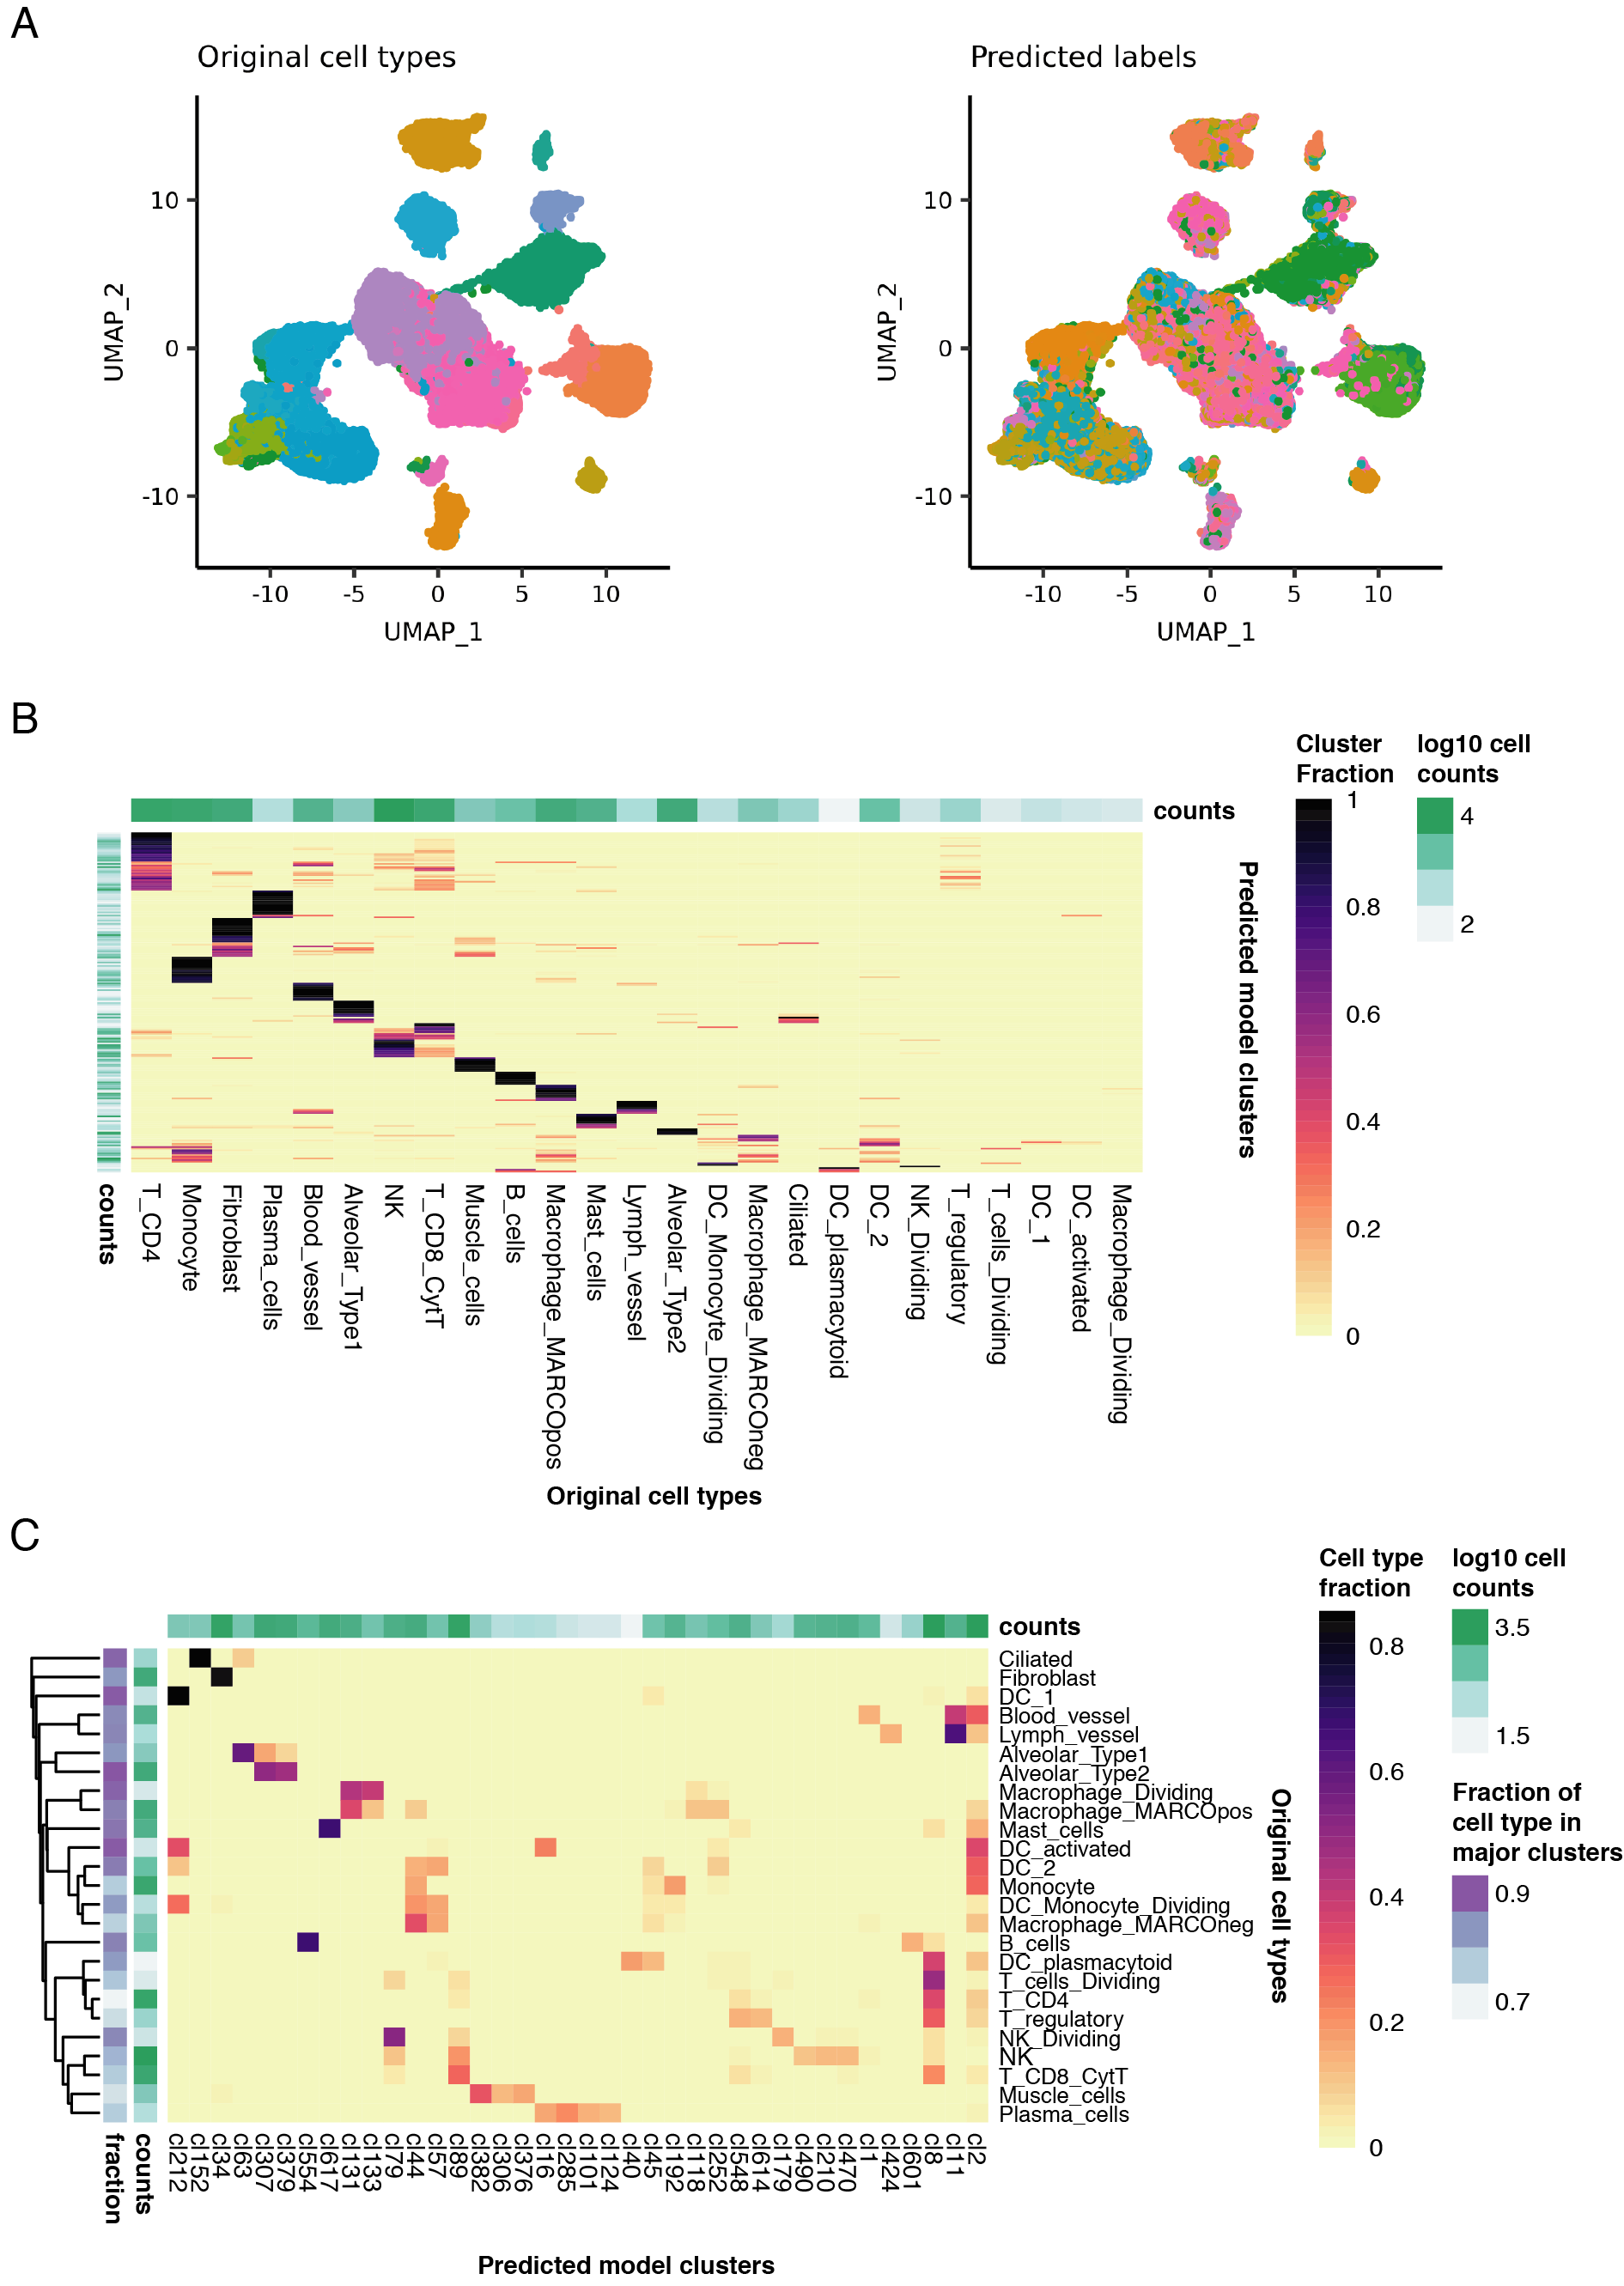
\includegraphics[scale=0.83]{Chapter4/Figs/chap4_preds.png} % change word in curlies to change figure
\caption[\textit{CellTypist} predictions for lung data from~\citep{madissoon_lung_2019}]{\textbf{\textit{CellTypist} predictions for lung data from~\citep{madissoon_lung_2019}}\newline\textbf{(A)} UMAP projections coloured by the original cell type annotations (left) and those predicted by \textit{CellTypist} (right) using thr1 = 0.99 and thr2 = 0.8. \textbf{(B)} Proportion of clusters (rows) matching each annotated cell type (columns). \textbf{(C)} Proportion of annotated cell types (rows) included in each cluster (columns). Only clusters including at least 10\% of a given cell type were included.}
\label{fig:chap4_preds}
\end{figure}

The data generated in~\citep{madissoon_lung_2019} was used to test the classification performance of \textit{CellTypist} with the compiled human data. This dataset was chosen because it includes three distinct tissues - lung, oesophagus, and spleen. Of the three tissues, lung is the only represented in the collected datasets (yet not contributed from the same sample), although many of the cells collected from spleen (mostly immune cells) are present in the model, contributed by different tissues. More than 200.000 cells were collected from these three tissues, with various cell populations manually identified.

An overview of the classification results, projected in UMAP~\citep{mcinnes_umap:_2018} (Figure~\ref{fig:chap4_preds}A, Figure~\ref{fig:appB_oes}A, Figure~\ref{fig:appB_spleen}A), shows a similarity between the individual labelling of different clusters. The increased noise in \textit{CellTypist}'s annotations are likely due to the large number of categories it includes. Despite this, most model labels are highly specific, being attributed almost entirely to a single original cell type annotation (Figure~\ref{fig:chap4_preds}B, Figure~\ref{fig:appB_oes}B, Figure~\ref{fig:appB_spleen}B). While the opposite is not true (i.e. one cell type annotation can correspond to more than one cluster), it is nonetheless evident that each cell type is dominated by one or very few clusters (Figure~\ref{fig:chap4_preds}C, Figure~\ref{fig:appB_oes}C, Figure~\ref{fig:appB_spleen}C). Furthermore, even when excluding clusters including less than 10\% of cells from each annotated cell type (as is the case in the heatmap in Figure~\ref{fig:chap4_preds}C), the remaining clusters still include 70-90\% of cells (purple sidebar in Figure~\ref{fig:chap4_preds}C). 

A downside of validating \textit{CellTypist} with independent data is that the comparison can not be directly assessed, since the existing annotations for this dataset do not match those used by \textit{CellTypist}, which compiles a variety of nomenclatures used in each specific publication from where the data was obtained. Nonetheless, this can be circumvented by manual inspection of existing labels, as well as matching the dataset annotations with the model clusters to approximate a gold standard.

\begin{figure}[pht!]
\centering
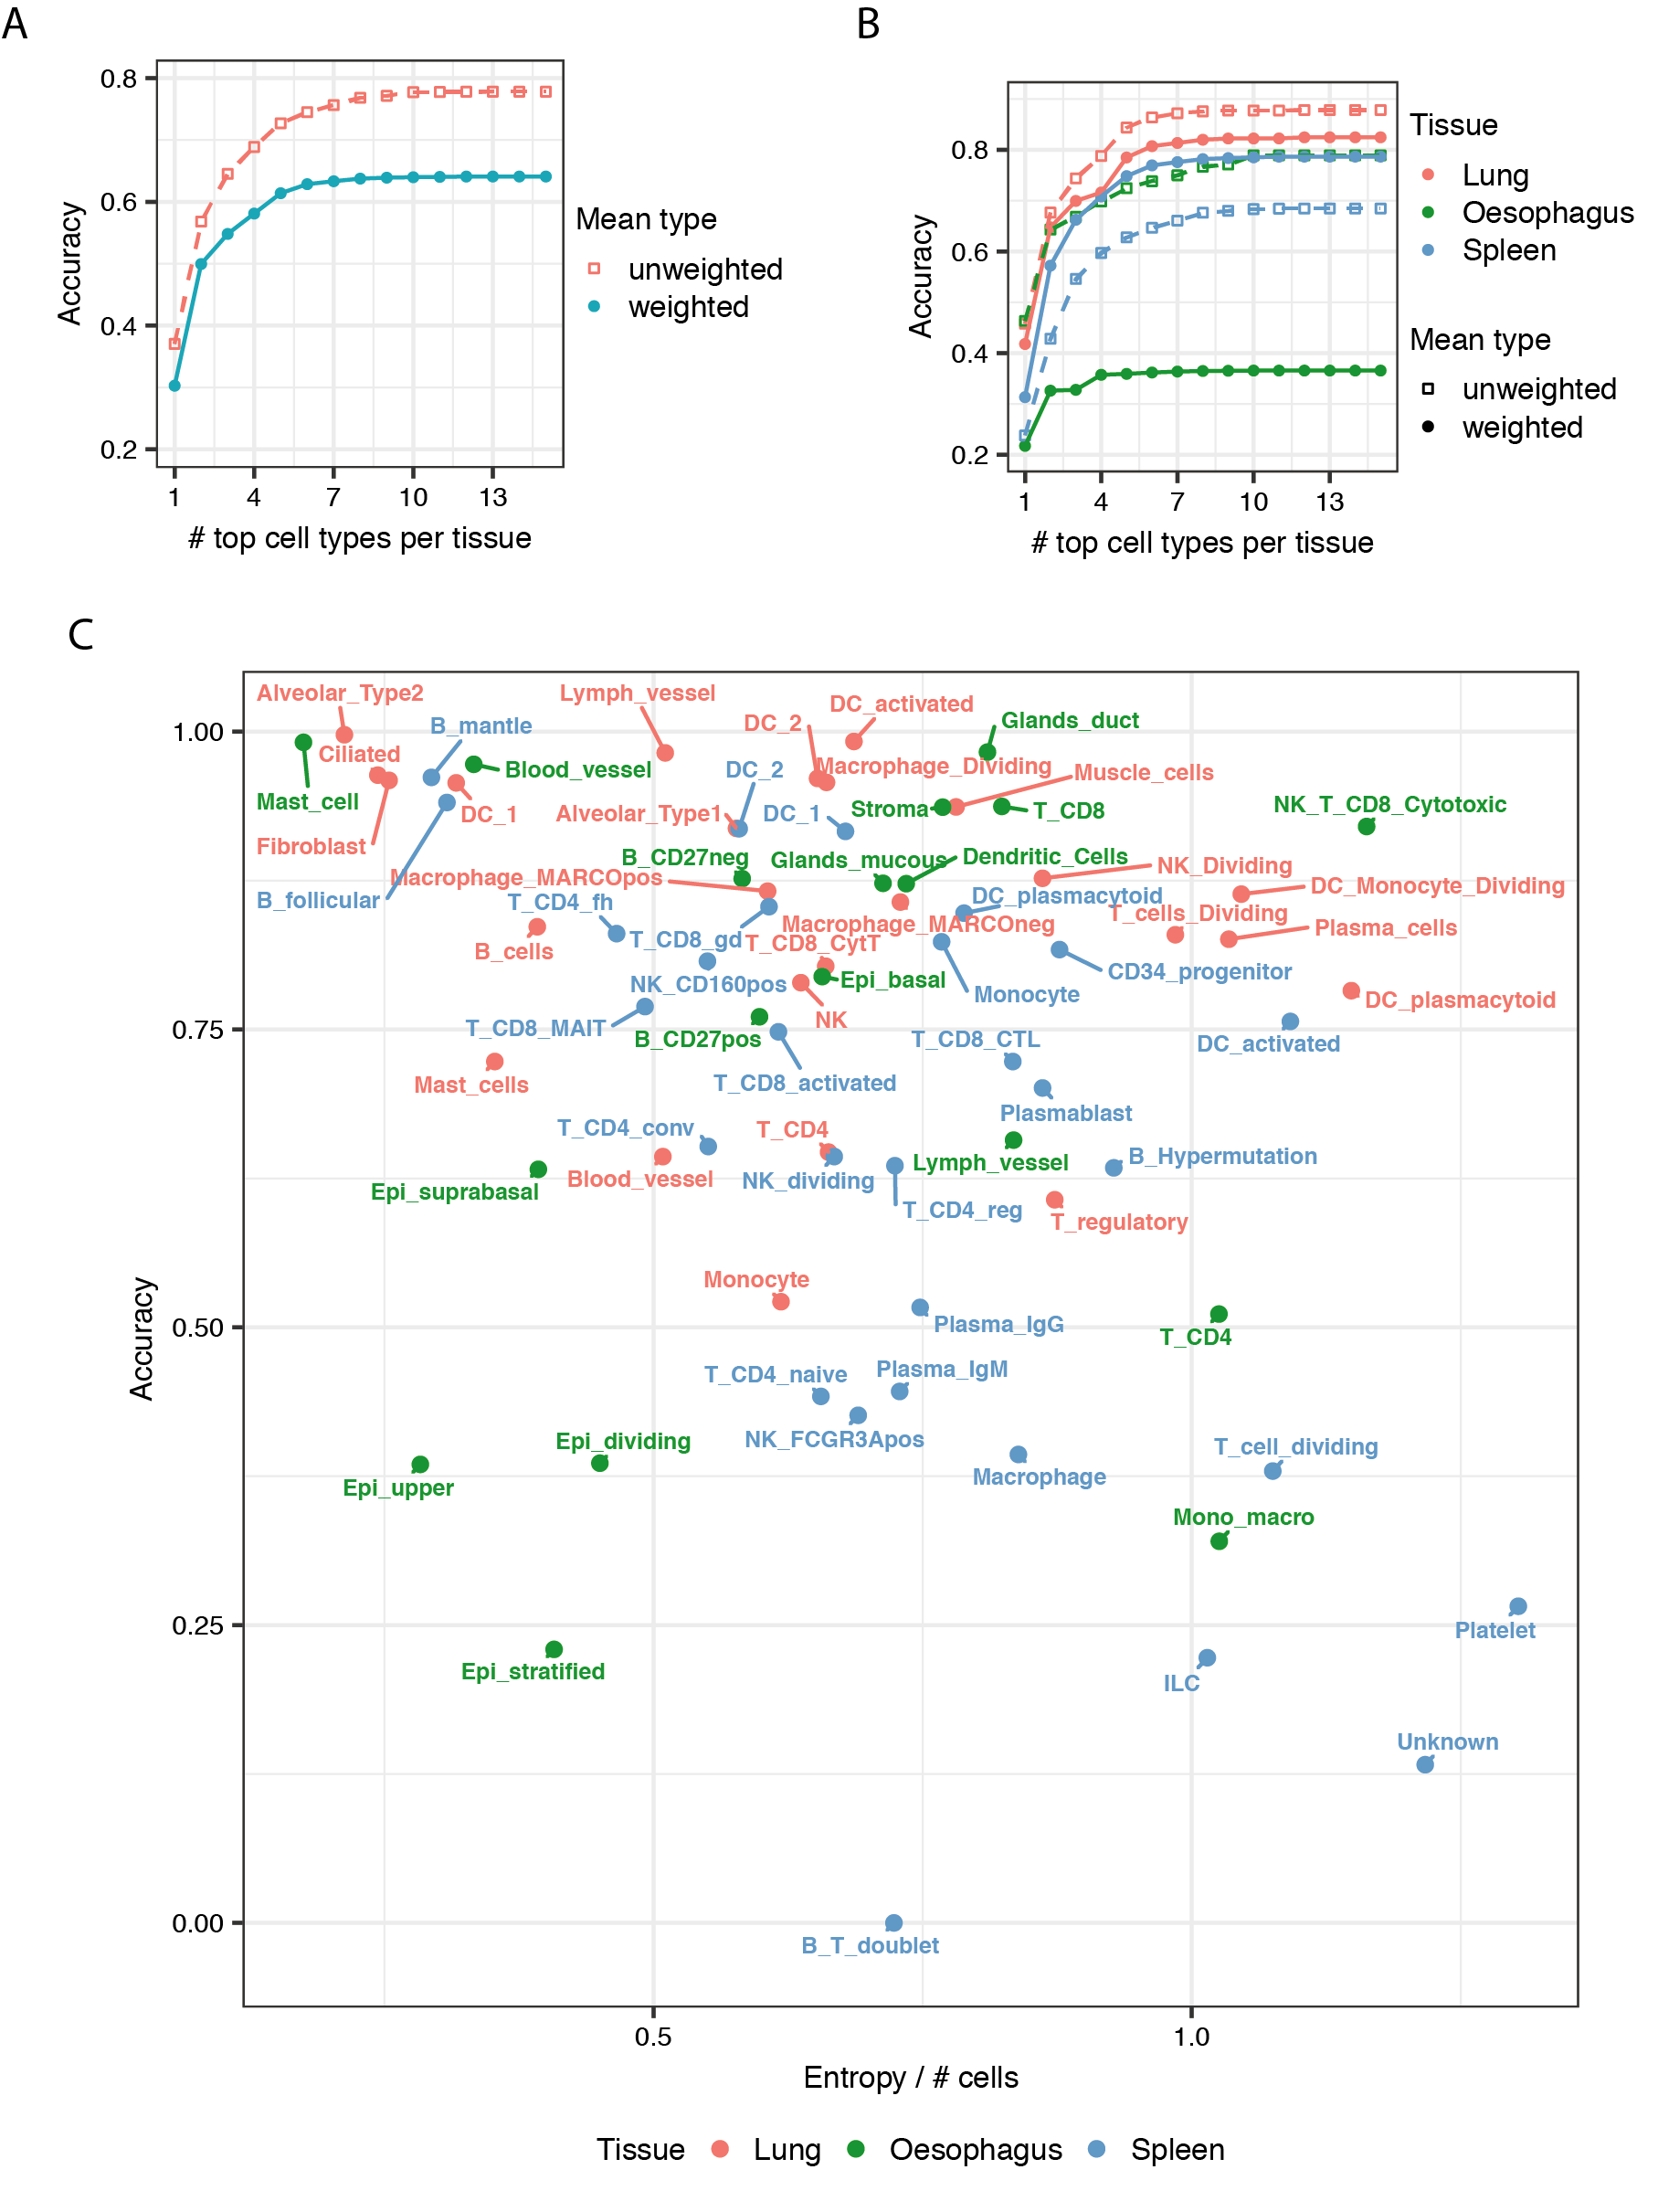
\includegraphics[scale=0.85]{Chapter4/Figs/chap4_madissoonAcc.png} % change word in curlies to change figure
\caption[Classification accuracy for the~\citep{madissoon_lung_2019} dataset]{\textbf{Classification accuracy for the~\citep{madissoon_lung_2019} dataset}\newline\textbf{(A)} Variation in mean accuracy with the maximum number of cell types from each tissue allowed to be matched to a cluster. Weighted mean takes the number of cells into account. \textbf{(B)} Variation in mean accuracy with the maximum number of cell types from each tissue allowed to be matched to a cluster, stratified by tissue. \textbf{(C)} Classification accuracy for each cell type from each tissue (colour), as a function of the entropy calculated for the predicted cluster representation of each cell type, normalised by its representation.}
\label{fig:chap4_accu}
\end{figure}

A more careful look at the annotations present in the clusters that matched each original cell type in lung reveals the accuracy of the model. Type 2 alveolar cells matched clusters only containing that same annotation, whereas clusters in alveolar type 1 included type 1, and type 2, as well as secretory cells. Ciliated cells and fibrolasts mostly matched a single cluster each, in both cases composed of the exact same annotation. Cells annotated as "Lymph\_vessels" and "Blood\_vessels" both matched cl11 (containing "endothelium" and "lymphatic" cells), with the first also matching lymphatic endothelial cells from the axillary lymph node. T cell annotations were mostly assigned to cluster cl8, which includes a mix of CD4 and CD8 cells. In addition, T regulatory cells also matched cluster cl614, which includes activated T cells and Tregs. NK cells also matched a cluster with CD8 T cell annotation, but included two others containing mostly NK cells from other tissues. Lung cells that are derived from the myeloid lineage (Macrophages, Monocytes, Dendritic cells) all matched clusters mostly composed of these same annotations, albeit with some mix between them, which again demonstrates some of the difficulty that exists in separating these cell types.

For a more quantitative assessment of \textit{CellTypist}'s accuracy, an identical cell type nomenclature would have to exist between the model and the validation dataset. While one could opt for renaming \textit{CellTypist}'s labels in accordance with those present in the model, two arguments invalidate this approach. First, converging into the exact same labels could be misleading, since different methodologies would be utilised for labelling the validation dataset and the model clusters - the latter would rely on the model coefficients, as well as existing annotation from the original datasets. Second, this would not take into account differences in resolution between the model and the data, and would penalise its lack of specificity. An example of this is the situation described in the previous paragraph for the dataset's "Lymph\_vessels" and "Blood\_vessels" labels, which both match a clearly general endothelial cluster, and thus opting for one of these labels would wrongly penalise the other.

Instead, correspondence between dataset cell types and model clusters was independently determined by assessing the enrichment for cell type markers in the top 500 coefficients for each model label using GSEA (see Methods Section~\ref{section4.4_genelists}). This was done in an attempt to approximate the annotations based on marker genes expression, the most commonly used methodology. All tissue/cell type combinations were tested together for enrichment, filtered for significance (q-value<=0.05) and positive enrichment scores, and ranked by the latter. Cluster-cell type correspondence was assessed per tissue, with a variable number of corresponding top cell types accepted (Figure~\ref{fig:chap4_accu}A and B). Accuracy was then calculated for each cell type, based on whether each cell's cluster assignment by the model had was enriched for the same cell type originally labelling that cell. As expected, inclusion of more cell types to match each cluster led to increasing accuracy (Figure~\ref{fig:chap4_accu}A). This accuracy was different between tissues, with lung as the best positioned, followed by Spleen and the Oesophagus (Figure~\ref{fig:chap4_accu}B). This is in line with the composition of the data that underlies \textit{CellTypist}: Lung has a high accuracy since this tissue and most of its cell types are represented; Spleen also has elevated scores since it is mostly composed of immune cells, which are highly abundant in the model coming from Blood, Bone Marrow, and other tissues; Oesophagus presents a lower score due to the fact that the sample mostly includes different types of specialised epithelial cells, which are absent or underrepresented in the model.

The accuracy per cell type and tissue was then examined (Figure~\ref{fig:chap4_accu}C), allowing for up to 5 cell types to correspond to a cluster, the value at which accuracy stabilises. These assignments can be found in Supplementary Table~\ref{table:tab_mad_match} to Supplementary Table~\ref{table:tab_mad_match9}. A value greater than 1 also has the advantage of allowing for a proper reflection of the many-to-many relationship that can exist between model clusters and manual cell type annotations. However, it should also be noted that this implies, in many cases, that the model cluster represent a lower resolution or broader cell type identity. This can be seen for example at the level of macrophages and other myeloid cells, where in many cases their (sub)types are enriched in the same cluster (for a concrete example, see cl252 in Supplementary Table~\ref{table:tab_mad_match2}). Figure~\ref{fig:chap4_accu}C shows an increased accuracy for most immune cell types, as well as lung-derived cells. The lowly-performing immune cells from the spleen originate from rarer populations, which explains the higher weighed mean accuracy, and reveals resolution limitations in the model. Inversely, most of the top performing cells from Oesophagus come from immune cell populations with a low level of specificity (as illustrated by the "NK\_T\_CD8\_Cytotoxic" label), which also make up a small percentage of the total cells recovered from this organ. We can also observe that there is a modest negative correlation between the accuracy for each cell type and how many clusters each cell type is distributed across (normalised by log10(number of cells), Spearman Correlation = -0.33, p-value<0.01). Lastly, from Figure~\ref{fig:chap4_accu} we can conclude that accuracy from represented cell types and tissues will be in the 0.4 to 0.85 range, and rare or absent cell populations will present an accuracy between 0.2 and 0.5.

% other models
The other models resulting from different parameters were also briefly examined. Despite the differences in number of clusters, all models show a similar specificity for the assigned clusters (Figure~\ref{fig:appB_othercl}). However, both models with fewer clusters (thr1 = 0.25, thr2 = 0.25; and thr1 = 0.1, thr2 = 0.1) both show less unique matching of original cell types to clusters (Figure~\ref{fig:appB_otherct}), with most of them matching the same larger clusters, which is likely an artifact of excessive merging within and across tissues (Figure~\ref{fig:chap3_combcl}A). 

Globally, it has been demonstrated that \textit{CellTypist} can be successfully used to annotate datasets with a broad diversity of cell types, and future improvements to the pipeline are likely to make it more precise in attributing cell identity. 


\subsection{Matching cell identity across tissues}
\label{section_tissues}
The clusters detected in each tissue are independent of the number of datasets (Spearman Rank Correlation = -0.01, p-value for null hypothesis of "${\uprho}$=0" = 0.9344), although moderately correlated with the number of cells present in each tissue (Spearman Rank Correlation = 0.52, p-value for null hypothesis of "${\uprho}$=0" = 0.01497) (Figure~\ref{fig:appB_clustnumbs}). The subsequent cluster merging step draws a map of cell identity relationships across tissues. Examining this map can reveal higher order relationships between the tissues present in the global dataset. Thus, the per-tissue classification probabilities used to construct the cluster matching graph (Figure~\ref{fig:chap3_combcl}A) were used to calculate the mean probability of cells from a per-tissue (non-merged) cluster matching the clusters of all tissues. The resulting tissue-by-cluster mean probability matrix is represented in the clustered heatmap of Figure~\ref{fig:chap4_tiss}A. This plot shows that about a third of all clusters have an average high confidence assignment across tissues (bottom of the heatmap), with the remaining two-thirds having much lower per-tissue mean probabilities. 

The clustering of these values reveals a stark division between tissues whose immune compartment was predominantly profiled (left major branch of dendrogramme), and those with a more global or non-immune profiling (right branch). This is highlighted by the per tissue mean expression of \textit{PTPRC}, the gene encoding for the CD45 receptor, which is exclusively expressed in immune cells~\citep{altin_role_1997} (Figure~\ref{fig:appB_ptprc}). Expression of \textit{EPCAM} - an epithelial cell marker - and \textit{CD34} - an endothelial cell marker - further illustrate this division, being most expressed in tissues in the opposite dendrogramme branch. The same effect, however, is not as pronounced when examining the results from the \textit{Tabula Muris} dataset (Figure~\ref{fig:chap4_tiss}C), where cell type sampling is less biased per tissue. Tissues with similar levels of expression of the same markers can be observed to cluster together (heatmap tissue clusters with AU p-value<=95: Spleen and Marrow; Trachea to Muscle; Kidney and Liver; Brain\_Neurons and Pancreas); however the stark immune/non-immune division observed for human data is no longer present. We can thus conclude that tissue similarity, as defined by cell type correspondence, is driven by cell identity, in particular by the major lineage (immune, epithelial, endothelial), yet can be affected by cell type sampling proportions.

\begin{figure}[pht!]
    \centering    
    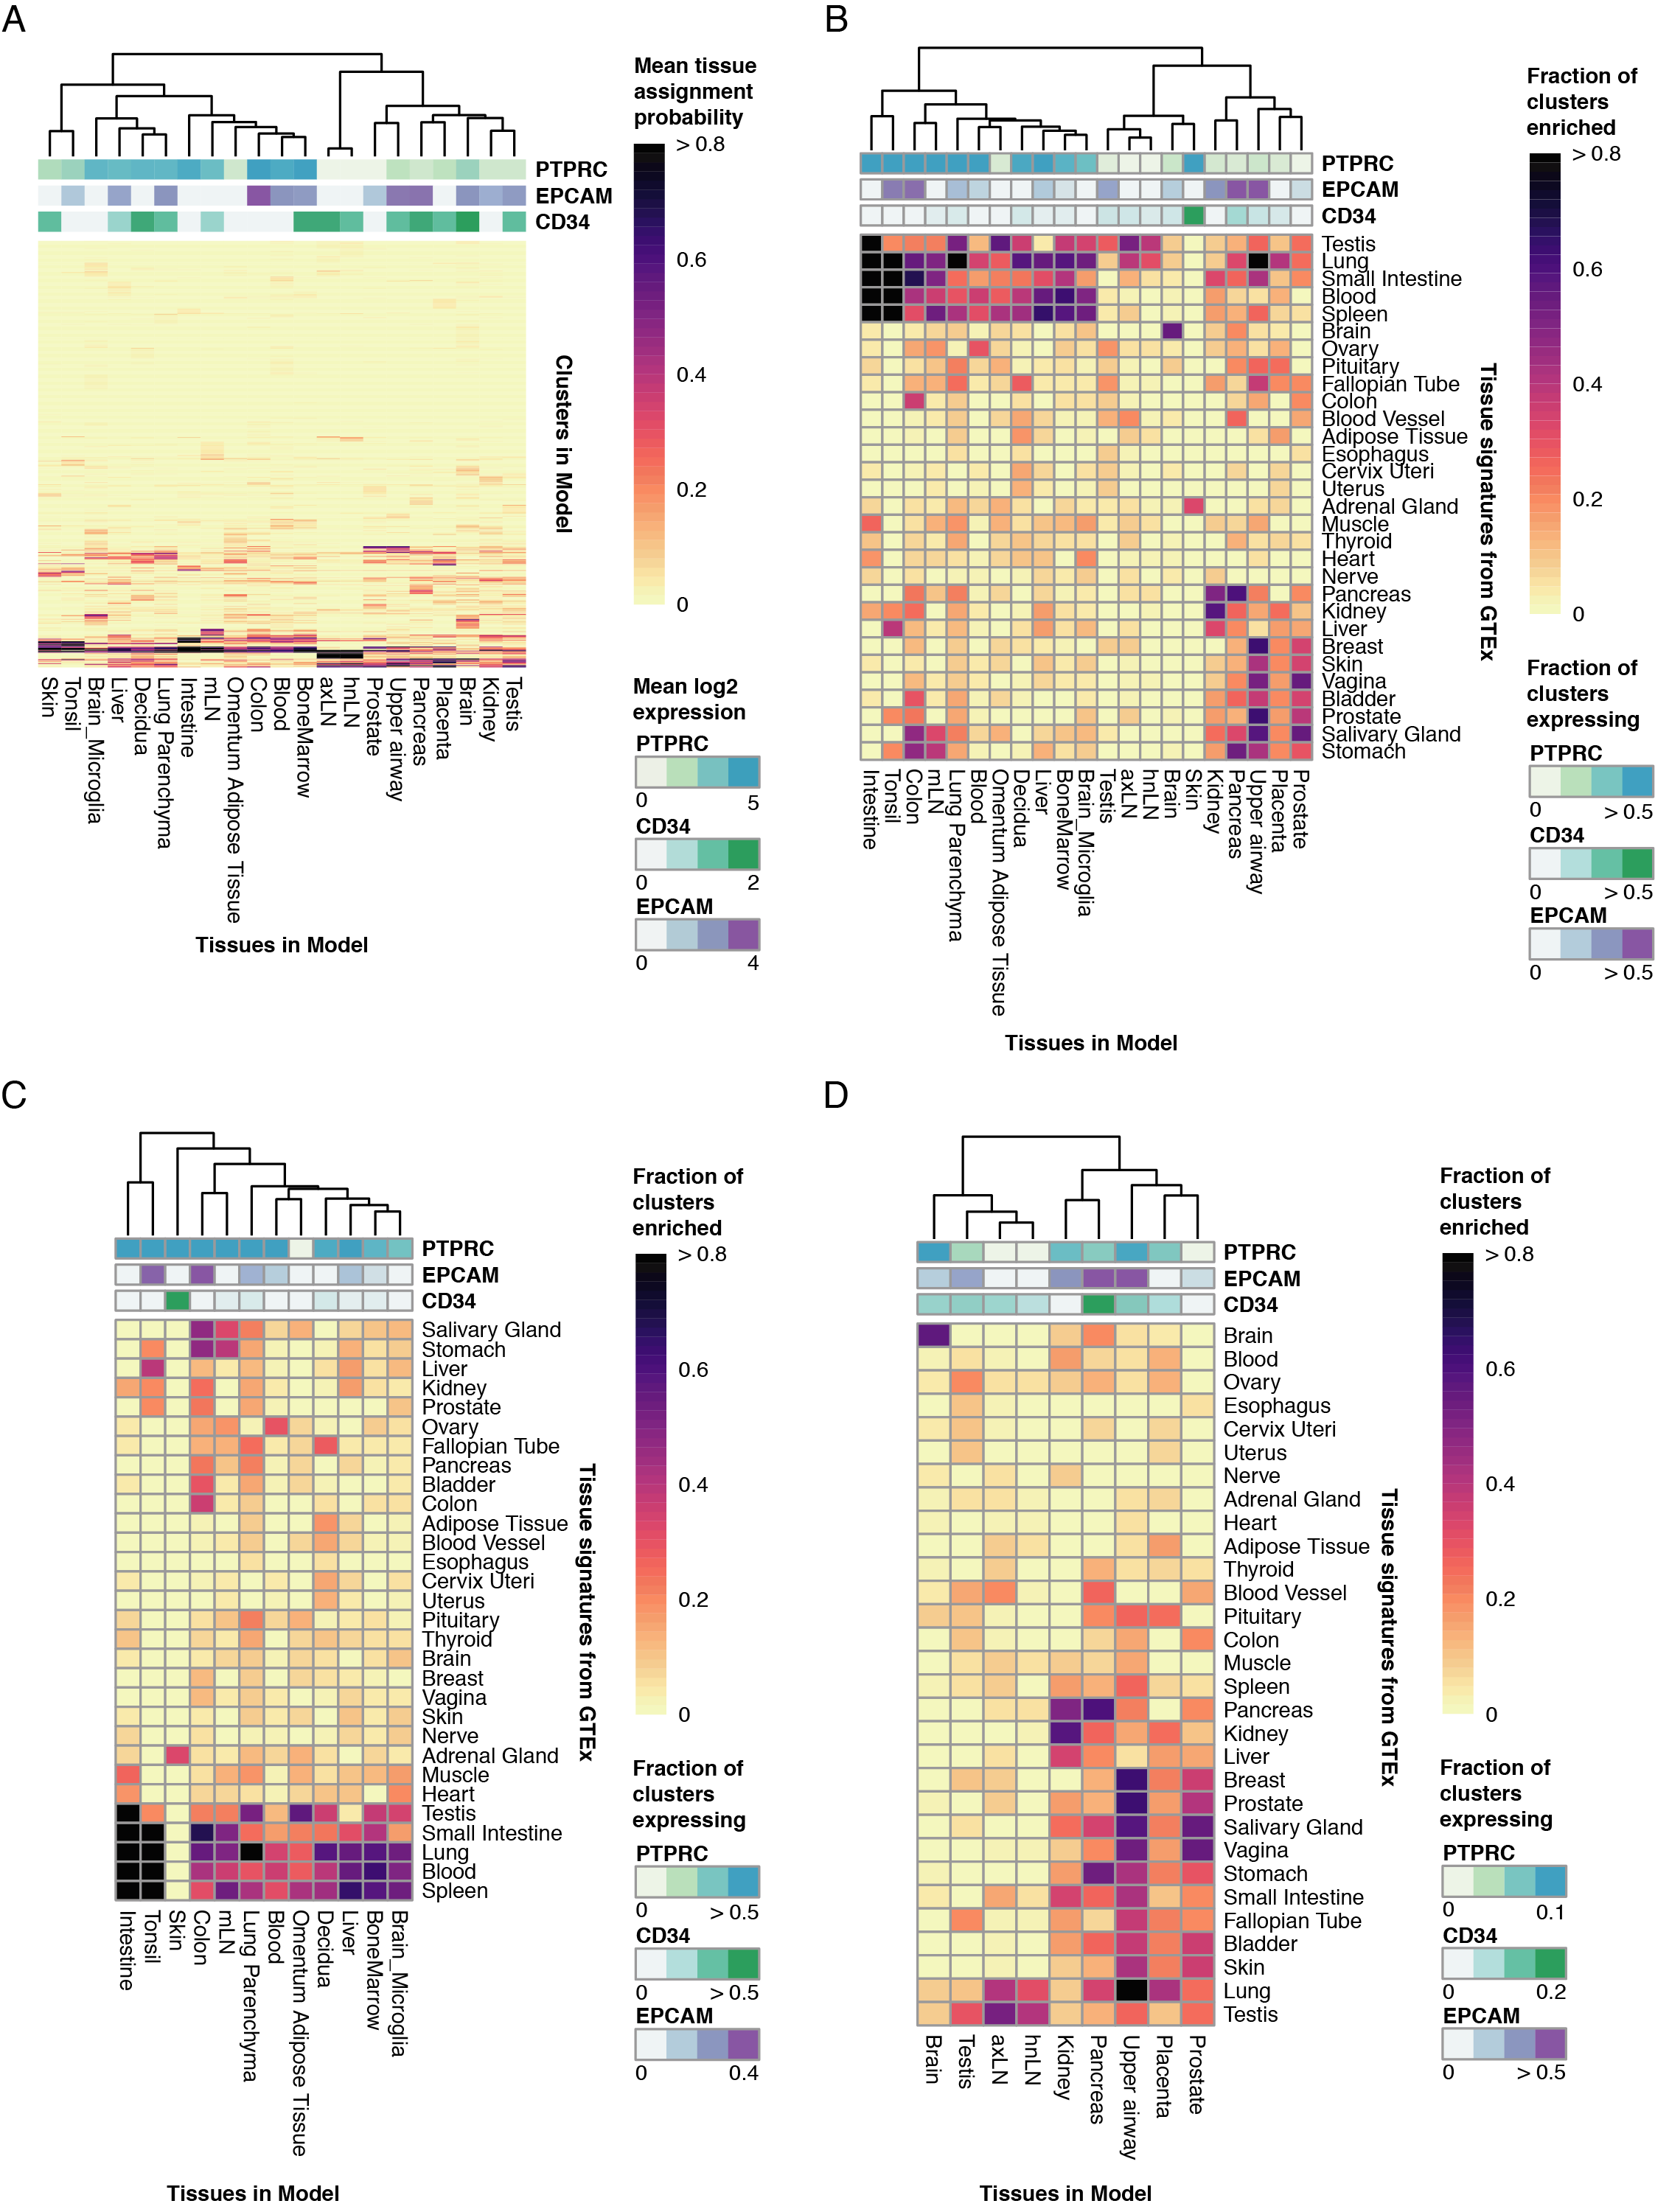
\includegraphics[scale=0.66]{Chapter4/Figs/chap4_tissuefig.png} % change word in curlies to change figure
    \caption[Cell identity relationships across tissues]{\textbf{Cell identity relationships across tissues}\newline\textbf{(A)} Heatmap of the mean assignment probability of cells from a per-tissue cluster to the clusters of each given tissue in the human collection dataset. \textbf{(B)} Heatmap of the fraction of human collection clusters from a given tissue whose \textit{CellTypist} model (thr1 = 0.99; thr2 = 0.8, see Chapter~\ref{chap:CT_method} Section~\ref{section3.3_human}) signature is enriched in certain tissue-specific genes. Gene signatures were derived from GTex bulk RNA-seq data. \textbf{(C)} Heatmap of the mean assignment probability of cells from a per-tissue cluster to the clusters of each given tissue in the Tabula Muris dataset. \textbf{(D)} Heatmap of the fraction of Tabula Muris clusters from a given tissue whose \textit{CellTypist} model (thr1 = 0.8; thr2 = 0.99, see Chapter~\ref{chap:CT_method} Section~\ref{section3.3_mouse}) signature is enriched in certain tissue-specific genes. Gene signatures were derived from ENCODE tissue bulk RNA-seq data.}
    \label{fig:chap4_tiss}
\end{figure}

Tissue identity is also reflected in gene expression, and therefore in the genes with the top coefficients determined by the \textit{CellTypist} model. To unbiasedly probe the existence of tissue-specific signatures in the top genes of all clusters, tissue signatures were derived from bulk RNA-seq data, using data from the GTEx Consortium for human~\citep{consortium_genotype-tissue_2015} and from the ENCODE Consortium for mouse~\citep{dunham_integrated_2012} (see Methods Section~\ref{section4.4_genelists}). This provided independent references for tissue identity using gene expression. Inspection of human tissue identity enrichment in cell clusters per tissue (Figure~\ref{fig:chap4_tiss}B) shows that, despite the sets of tissues in the \textit{CellTypist} and GTEx datasets not overlapping completely, matching between them is mostly concordant. Most immune cell-enriched tissues cluster independently (AU p-value = 96 for both branches) by having many clusters enriched in blood and spleen-specific genes. Beyond this separation, There is a high correspondence between tissue-specific genes and the tissues present in the data. Examples are Liver, Brain, Testis, Lung (Parenchyma), Kidney, Pancreas, and Colon (matching Small Intestine). Among the tissues with more diverging matching are Skin, likely because of the very biased cell sampling (Treg and Tmem cells~\citep{miragaia_single-cell_2019}). Other tissue correspondences might derive from functional similarities, such as Pancreas and Pituitary (hormonal secretion), Tonsil and Spleen (lymphoid tissues), or Upper Airway and Vagina (mucosal epithelia).

Similar specificity relationships can be observed in the \textit{Tabula Muris} dataset (Figure~\ref{fig:chap4_tiss}D), with a high matching for Pancreas, Liver, Kidney, Bladder, Thymus, and Lung, among others. Matching by functional or cell composition similarity was also present, such as Fat and mammary gland, or Diaphragm and skeletal muscle tissue. However, the evident division between immune/non-immune visible in human was once again absent. This further indicates that tissue composition analysis at the single-cell level must be calibrated by cell composition, in order to avoid biased characterisations.

The tissue relationships highlighted by the gene set enrichment directly derive from the \textit{CellTypist} model trained and the cell groupings that the pipeline defines. Examining other model alternatives shows that in some of them the tissue hierarchy is maintained (Figure~\ref{fig:appB_tissGSEA}), with the exception of the thr1 = 0.1, thr2 = 0.1 model. This is likely caused by excessive merging of clusters, leading to non-meaningful groupings and not so meaningful gene coefficients from the model.

%paragraph about the matching clusters
Plotting the clusters resulting from cross-tissue merging in \textit{CellTypist} can also reveal the similarity across tissues (Figure~\ref{fig:appC_tissrel}). As already shown by Figure~\ref{fig:appB_grids}A, the model with thr1 = 0.99 and thr2 = 0.8 is the one with the lowest number of merged clusters. We can however still observe clusters merging across tissues that have similar profiles and were included in the "immune enriched" group in Figure~\ref{fig:chap4_tiss}B - liver and bone marrow, lung parenchyma and intestine, decidua and omentum adipose tissue - as well as tissues that have functional associations - decidua and placenta, upper airway and lung parenchyma. The remaining models appear to maintain the occurrence of these associations between tissues, like the close clustering between axLN and hnLN, or the association of tissues including more immune sampling with blood and bone marrow. This is further underscored when the tissue gene signatures are examined in the merged clusters of each model (Figure~\ref{fig:appB_clmGSEA}). Both thr1 = 0.4 and thr2 = 0.99 and thr1 = 0.25 and thr2 = 0.25 again present the distinctive pattern of clustering the tissue signatures by the tissue functions as described before for the immune/non-immune partitions. The first model (thr1 = 0.99 and thr2 = 0.8) also shows some of this pattern, although not as evidently, likely due to the lower number of merged clusters. The same can not be observed for the thr1 = 0.1 and thr2 = 0.1 model, likely due to excessive merging leading to a less meaningful classifier.

Together, these results show that single cell populations in different tissues capture some of the tissue biology and specificity, representing functional and compositional relationships between them.


\subsection{Gene expression hallmarks of cell identity}
\label{section_genes}
The training of a logistic regression-base classifier model as used in \textit{CellTypist} allows for a direct evaluation of the genes important for the classification of each cluster through their learned coefficients. With a comprehensive cell type reference, we can start to unravel what are the key determinants of cell identity across tissues.

\begin{figure}[pht!]
    \centering
    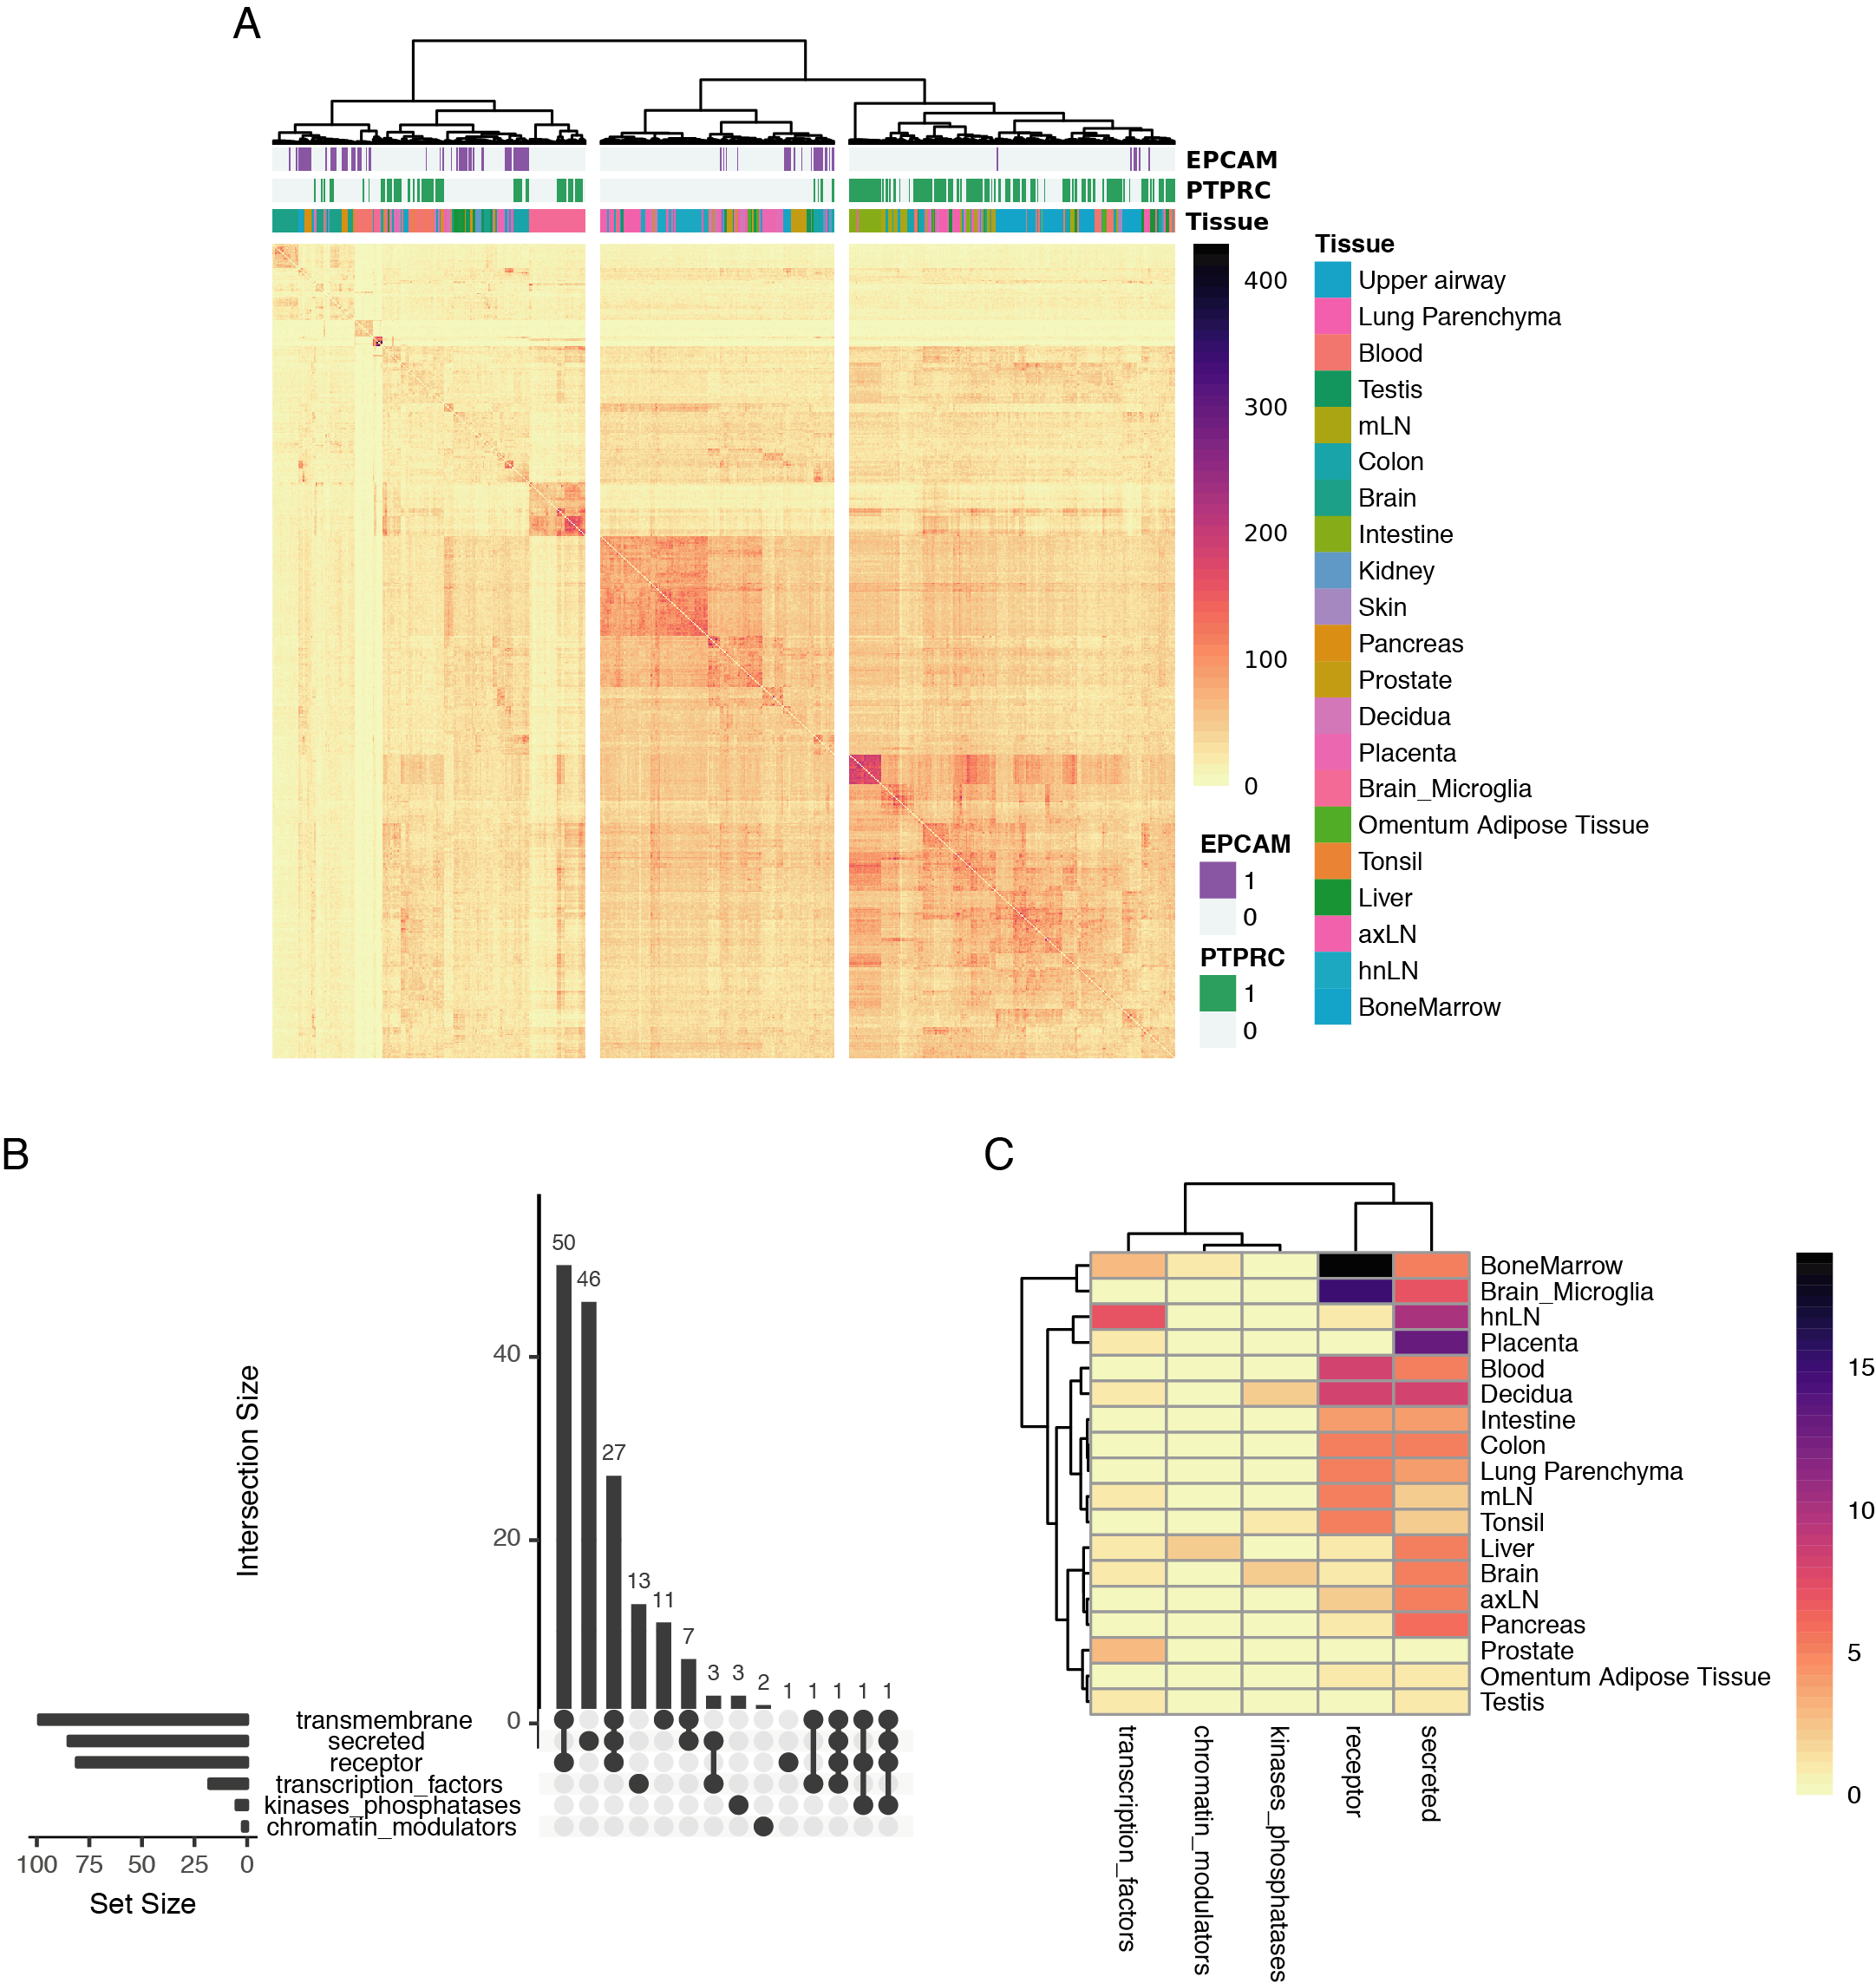
\includegraphics[scale=0.835]{Chapter4/Figs/chap4_genesAnalysis.png} % change word in curlies to change figure
    \caption[Top gene groups for cell identification across human tissues]{\textbf{Top gene groups for cell identification across human tissues}\newline\textbf{(A)} Clustered heatmap of the number of genes in common between pairs of \textit{CellTypist} clusters (thr1 = 0.99, thr2 = 0.8) in human data. Genes per cluster were determined as those with the top 500 coefficients learned by the model. Values in the diagonal (number of genes per cluster, 500) were set to 0. \textbf{(B)} Upset plot counting the number of clusters enriched for a group of genes with a specific function. \textbf{(C)} Heatmap of number of clusters per tissue (y-axis) enriched for groups of genes with a specific function (x-axis). For panels (B) and (C), the gene groups "transcription factors", "transmembrane", "secreted", "receptors", "membrane peripheral proteins", "kinases and phosphatases", "chromatin modulators", "catalytic enzymes", "housekeeping genes" were tested. Only the terms enriched in at least one cluster are shown.}
    \label{fig:chap4_genetypes}
\end{figure}

\begin{figure}[pht!]
    \centering
    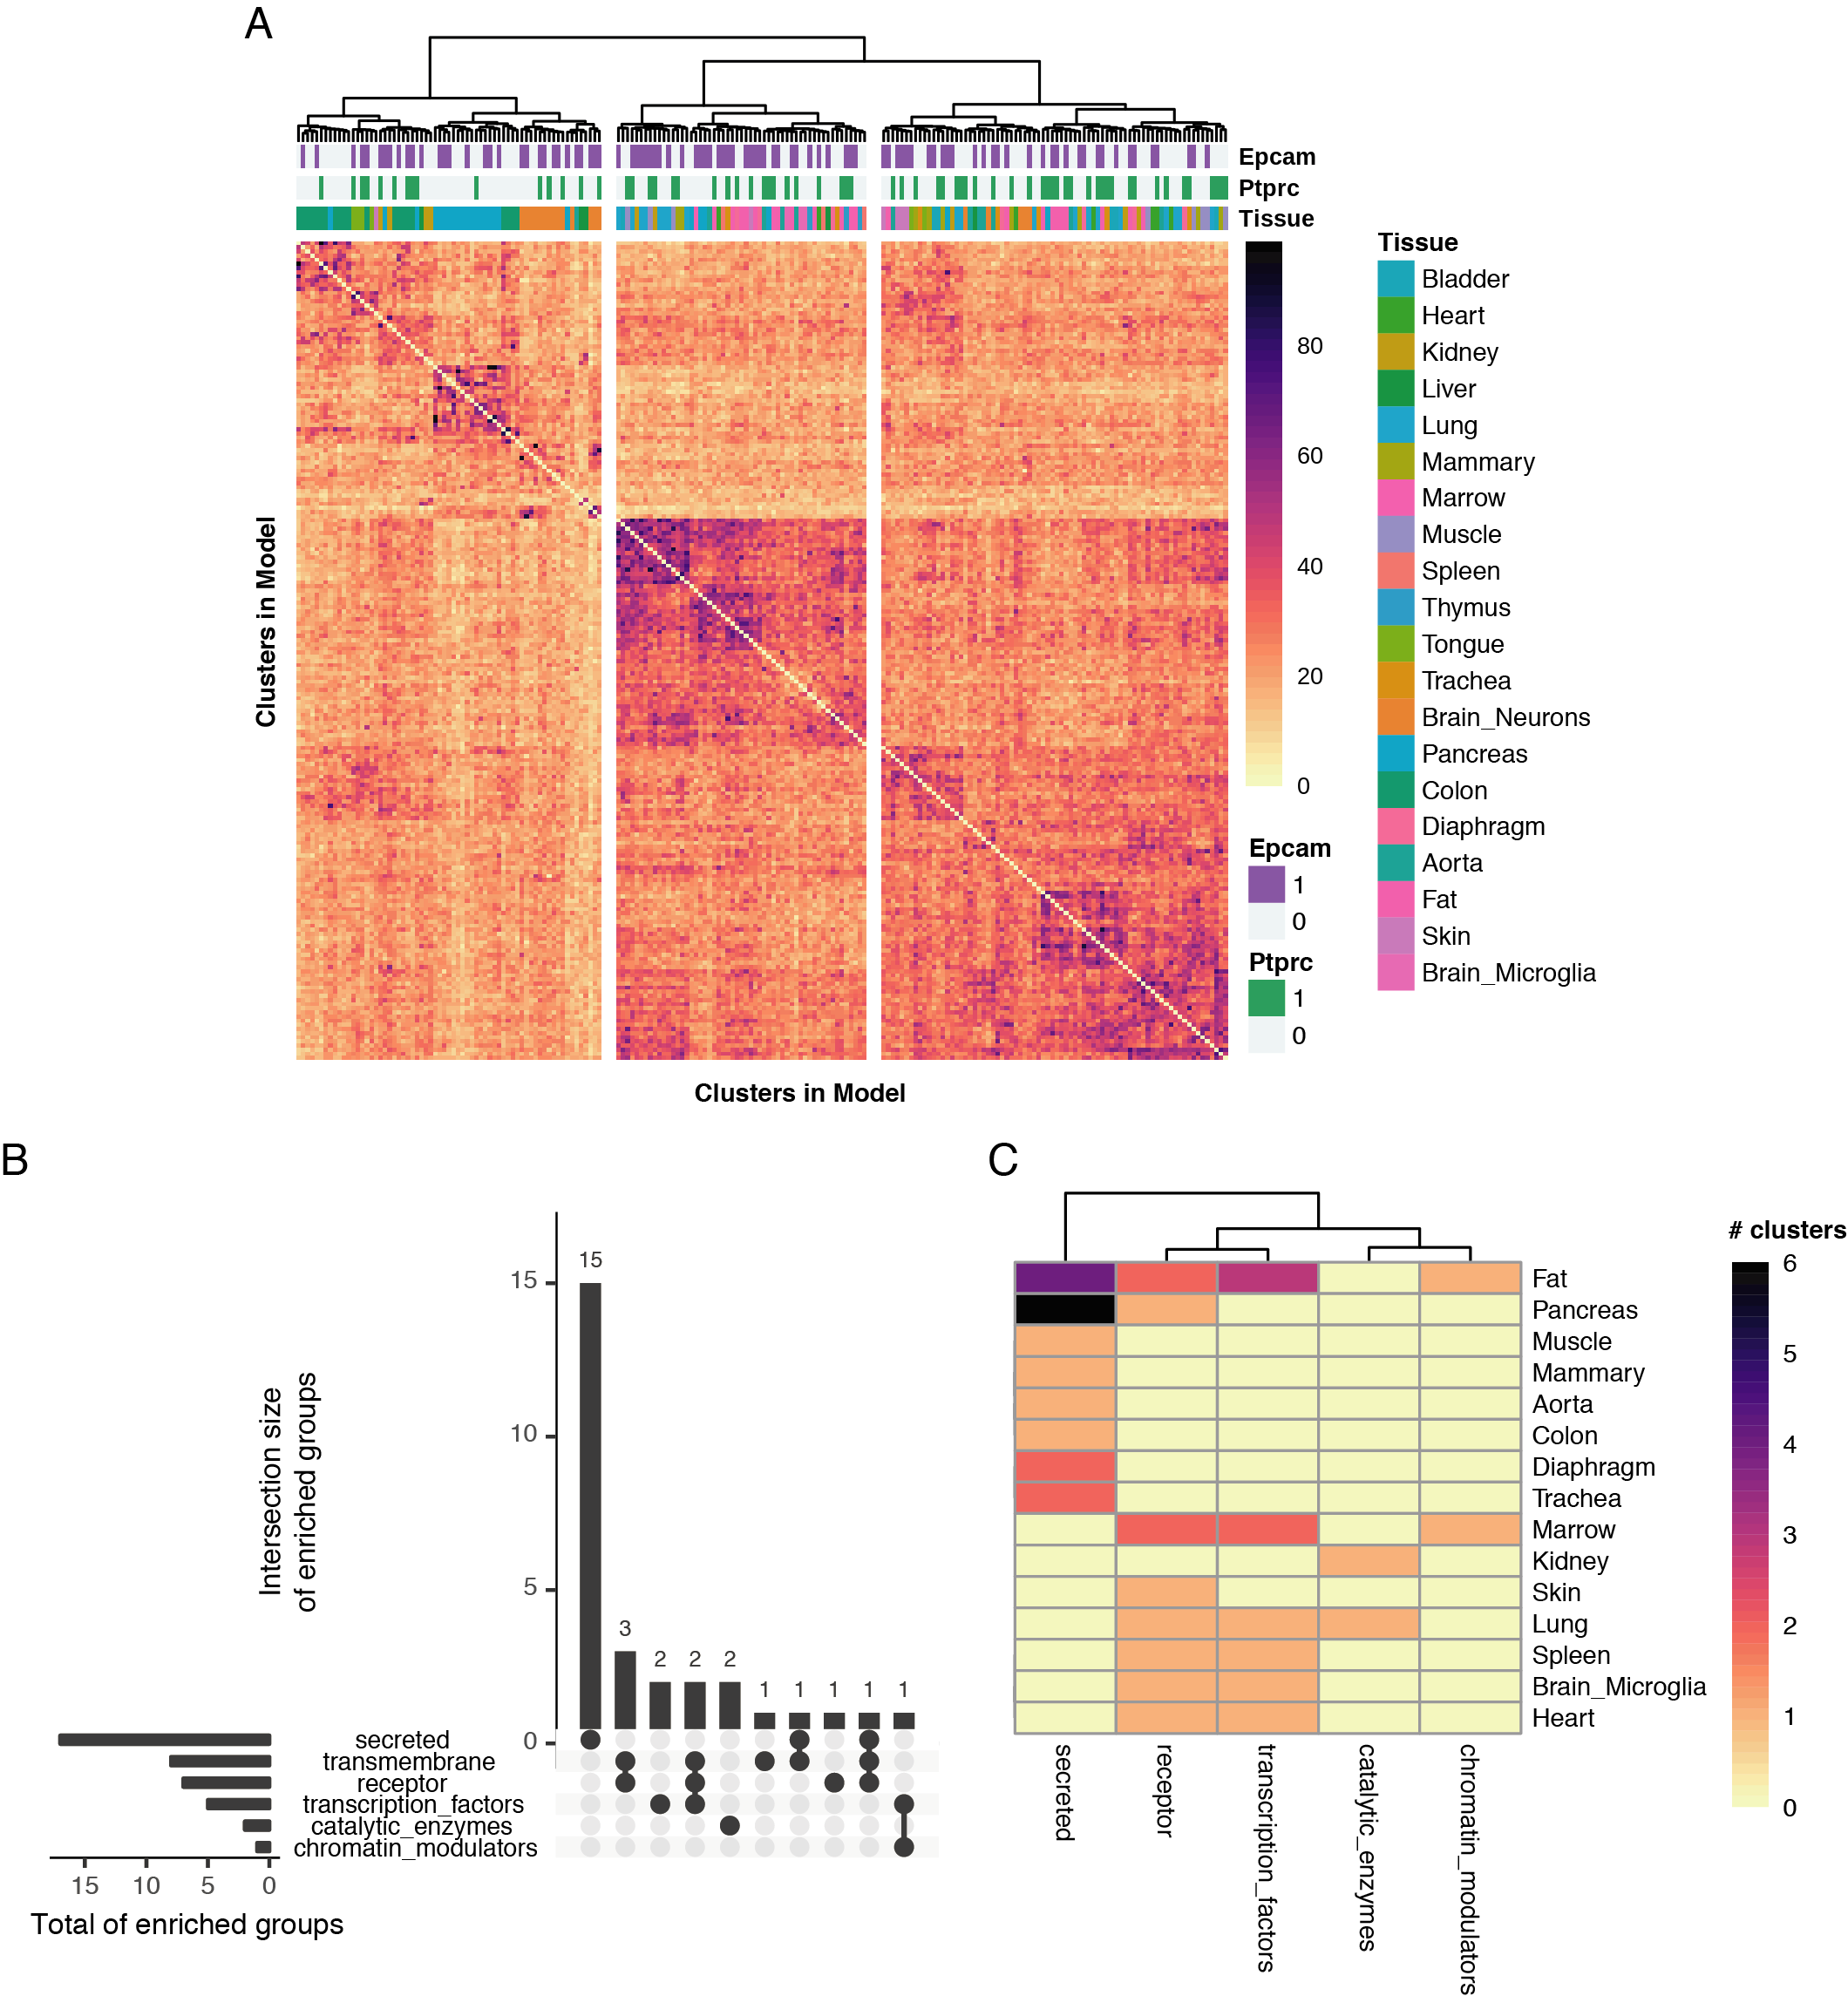
\includegraphics[scale=0.835]{Chapter4/Figs/chap4_genesAnalysis_mouse.png} % change word in curlies to change figure
    \caption[Top gene groups for cell identification across mouse tissues]{\textbf{Top gene groups for cell identification across mouse tissues}\newline\textbf{(A)} Clustered heatmap of the shared number of genes between pairs of \textit{CellTypist} clusters (thr1 = 0.8, thr2 = 0.99) in the \textit{Tabula Muris} data. Genes per cluster were determined as those with the top 500 coefficients learned by the model. Values in the diagonal (number of genes per cluster, 500) were set to 0. \textbf{(B)} Upset plot counting the number of clusters enriched for a group of genes with a specific function. \textbf{(C)} Heatmap of number of clusters per tissue (y-axis) enriched for groups of genes with a specific function (x-axis). For panels (B) and (C), the gene groups "transcription factors", "transmembrane", "secreted", "receptors", "membrane peripheral proteins", "kinases and phosphatases", "chromatin modulators", "catalytic enzymes", "housekeeping genes" were tested. Only the terms enriched in at least one cluster are shown.}
    \label{fig:chap4_genetypes_mouse}
\end{figure}

Relationships between human cell clusters were probed by counting the number of pairwise shared genes. The top 500 genes were used to avoid a hard coefficient value threshold across clusters, since the top values can be very variable between them. Clustering once more revealed a division between most immune and non-immune clusters (Figure~\ref{fig:chap4_genetypes}A). Moreover, various clusters containing cells from the same tissue were also grouped together, hinting at the existence of gene expression programmes shared by the different cell types within a tissue. 

The concept of "cell type" is still inconclusively defined, yet it can be intimately related to a cell's molecular phenotype, i.e. the molecules involved in cellular function. These can either be the effector molecules directly responsible for the cell's array of functions, or the genomic regulators controlling the expression of genes involved in these functions. It has been showed that tissue-specificity at the gene expression level is mostly due to transcription factor-gene regulatory interactions~\citep{sonawane_understanding_2017}. The \textit{CellTypist} model was used to assess what types of genes were more often at the top of the model coefficient rankings, which reflect the importance of expression of that gene in classifying a cell type. The following gene categories were considered (see Methods Section~\ref{section4.4_genelists}): Transcription Factors, Chromatin Modulators, Kinases and Phosphatases, Ligases and Deubiquitinases, Catalytic enzymes, Housekeeping genes, Receptors, Secreted proteins, Transmembrane proteins, and Peripheral membrane proteins. 

Both in human (Figure~\ref{fig:appB_human_coeff_exp}) and mouse (Figure~\ref{fig:appB_mouse_coeff_exp}), we did not observe a large difference between the mean expression levels of genes from different groups, or between their maximum coefficients, and most highly ranked genes (in the top 500) had a mean expression level around 10 reads. This coincided with a large correlation (0.56 in human, 0.86 in mouse, Spearman correlation coefficient) between mean expression and maximum reported coefficient, suggesting a dependency between expression level and gene importance for classification. However, this relationship appears to be non-linear, as evidenced by its shape which remains constant for genes with about 10 reads or more, and by the low Pearson Correlation Coefficient (0.05 in human, 0.08 in mouse). Thus, it can be inferred that gene importance for the model is only dependent of expression at low count levels.

Testing the gene groups described above for enrichment (see Methods Section~\ref{section4.4_enr}) showed a consistent pattern for all surveyed models of predominantly enriched membrane and secreted proteins (Figure~\ref{fig:chap4_genetypes}B, Figure~\ref{fig:appB_supupset}). A number of clusters also had transcription factors enriched in their top hits, albeit in markedly lower number. Enrichment for the tested gene groups appeared evenly distributed across tissues, and did not group them in any meaningful manner (Figure~\ref{fig:chap4_genetypes}C). Lastly, it is also notable that only a fraction of the total clusters showed enrichment for any of the classes tested, which could be due to the restrictive test that only looks for enrichment at the very top genes, as well as the non-comprehensive list of functions tested.

Examining the model produced by \textit{CellTypist} on the \textit{Tabula Muris} dataset revealed similar results. The grouping of immune versus non-immune clusters present in human was again absent (Figure~\ref{fig:chap4_genetypes_mouse}A), as had been observed in the previous Section (Figure~\ref{fig:chap4_tiss}). The patterns for gene groups were nonetheless similar, with a greater enrichment of secreted proteins across all cell clusters (Figure~\ref{fig:chap4_genetypes_mouse}B), and the largest significant groups spread across more various tissues (Figure~\ref{fig:chap4_genetypes_mouse}C).

These results point to the greater importance of the gene expression regulatory network's output molecules (genes coding for membrane and secreted proteins), when computationally defining the identity of a cell.


\section{Discussion}
\label{section4.3}
From its inception, the Human Cell Atlas (HCA) consortium has aimed to "define all human cell types in terms of distinctive molecular profiles (such as gene expression profiles)"~\citep{regev_human_2017}, a task that can not be easily accomplished by a single team. Beyond the financial and ethical constraints, collecting good quality scRNA-seq data requires tissue-specific knowledge, as well as profiling using both top-down and bottom-up approaches to obtain an overview of cell populations, while capturing cell type-specific phenotypic variations. Yet as data on human cells accumulates, methods capable of compiling the cellular census envisioned by the HCA members, and making it available to the community will be of great use.

% bias in collected data
%% model updating with new data will make it more inclusive/globally applicable
%% over represented cell types might "hide" smaller ones
%% data augmentation/downsampling can help
The human data presented provides a broad overview of several organs. This leads the cell type reference generated by \textit{CellTypist} to be broadly applicable to new datasets. This reference is dependent on the way these tissues are sampled. Currently, many of them are mostly or totally composed of immune cells which, while adding valuable information about their diverse phenotypes, can also bias the model. Collecting more datasets is the ideal way of mitigating this problem, but it can also be addressed by using data augmentation or downsampling approaches~\citep{wong_understanding_2016,hie_geometric_2019}. This would be especially relevant at the model training step, as we have observed the clear impact of number of cells per label in classification accuracy (Figure~\ref{fig:chap3_model}C, Figure~\ref{fig:chap3_modelcl}C, Figure~\ref{fig:chap3_HA}D).

Consistent data integration is also essential to avoid redundant classes and misleading interpretations about cell type and tissue relationships. Data integration for scRNA-seq is still a heavily studied topic~\citep{haghverdi_batch_2018,lopez_deep_2018,polanski_bbknn:_2019, stuart_comprehensive_2019}, and can considerably influence the cell groupings detected in the data. \textit{CellTypist} is likely to evolve as a pipeline, in order to adopt a within- and cross-tissue integration framework that closely reflects the cell type information available for each dataset. This integration will also lead to a clear cell type label for the model, while also reflecting the cell type resolution limitations of the classifier.

%tissue biology
Tissue identity relationships appear as an emergent result from the application of \textit{CellTypist}. The associations revealed between tissues are present at the cross-tissue integration stage (Figure~\ref{fig:chap4_tiss}A), and then also reflected in the top genes learned by the logistic regression model (Figure~\ref{fig:chap4_tiss}B). Furthermore, tissue identity is to some degree robust to incorrect or excessive grouping of single-cells (Figure~\ref{fig:appB_tissGSEA}), which reveals that tissues-specific expression programmes might be intrinsic to the core cell identity. The resolution of these tissue connections and programmes can be improved by broader cell type sampling and integration. This will allow the model to reveal a more fine-grained hierarchy beyond the immune/non-immune split, and ultimately map cellular phenotypes to a structured cell identity atlas.

% gene biology
%% more detailed conclusions can be taken once the reference is uniformly annotated/if more annotated data is included (because we can now go beyond tissues/clusters to actual cell types)
%% discuss how more accurate gene groups can give more accurate results
The data compiled offers for the first time a window into the gene expression hallmarks of cell identity. Analysis of enriched gene expression programmes can be improved by using a more uniform gene reference, as well as adopting more informative labels for the clusters obtained (which can come from improved dataset merging or manual annotation). Nonetheless, the analysis showed consistently ranked receptors and secreted molecules above transcription factors when defining cell identity (Figure~\ref{fig:chap4_genetypes}B, Figure~\ref{fig:appB_supupset}). This is in agreement with previous reports~\citep{sonawane_understanding_2017}, yet this is the first instance where this type of analysis could achieve this level of cell type resolution. Importantly, defining which genes make up the core of cellular phenotypes is not the same as defining cell identity regulation. However, knowledge of the minimal gene expression set required to classify or obtain a determined phenotype (and consequently function) is a key point in understanding the operational definition of cell types. Thus, the expansion and improvement of the \textit{CellTypist} reference will increasingly provide a foundation to understanding how cell types arise and evolve~\citep{zimmermann_ancient_2019}, and will help prioritise gene targets for effective cellular engineering.

% use and availability of this data collection
This large human cell type reference can be very useful to characterise cell identity in a variety of systems. In disease-focused studies, the steady-state reference provided by \textit{CellTypist} can automatically annotate the cells obtained from a disease sample, without relying on a matching healthy sample. This is useful in large scale studies that aim to quantify cell number alterations in disease, yet steady-state cells would still be required to identify disease-specific gene expression programmes or cell subpopulations. Another potential use is to characterise cell fates and heterogeneity when differentiating organoids. Classifying scRNA-seq data from the generated organoids using an unbiased reference can reveal the cell types present that a specific protocol was able to differentiate. \textit{CellTypist} will also be available as an online resource, where the model can be directly used, and is accompanied by a database showing the defining characteristics of each cell type - marker genes detected, tissues of origin, datasets characterising them, and similar cell types. This is further intended to be articulated with a Cell Ontology~\citep{bard_ontology_2005}, and have cell names be consistently used when new data is produced, with a direct correspondence to both databases. Lastly, future releases of \textit{CellTypist} models will include more species, adding an evolutionary layer to our knowledge of cell identity.


\section{Methods}
\label{section4.4}
\subsection{\textit{CellTypist} parameter optimisation and training}
\label{section4.4_model}
Use of the integration and model training pipeline in the human dataset collection was done as described in Chapter~\ref{chap:CT_method} Section~\ref{section3.3_human}, and is again briefly explained here. Data from the same tissues was integrated and clustered using the Leiden algorithm~\citep{traag_louvain_2019} at several resolutions. For tissues with cell type annotations, resolution was optimised using the split-join distance~\citep{dongen_performance_2000} between clusters and cell type annotation and constrained to a number of clusters at least as large as the number of cell type annotations in the largest collected dataset (Figure~\ref{fig:chap3_HA}A).

Following clustering, per tissue logistic regression models were trained, running for 10 epochs of a maximum of 100 iterations each. These models were used to run the cross-tissue cluster merging pipeline (Chapter~\ref{chap:CT_method} Section~\ref{section3.2.2}), and a combination of parameters was chosen based on the ratio of split-join distances (merged vs annotated cell types over per tissue vs annotated cell types) (Figure~\ref{fig:chap3_HA}B), resulting in the choice of thr1 = 0.99 and thr2 = 0.8. Additionally, three other combinations were chosen for comparison: thr1 = 0.4 and thr2 = 0.99, the combination with the top split-join ratio when only considering merged clusters (Figure~\ref{fig:appB_grids}C, Figure~\ref{fig:appB_moremodels}A-B); thr1 = 0.25 and thr2 = 0.25, one of the combinations with the highest fraction of merged clusters (Figure~\ref{fig:appB_grids}B, Figure~\ref{fig:appB_moremodels}C-D); thr1 = 0.1 and thr2 = 0.1, the combination with the highest fraction of merged clusters, as well as highest split-join fraction (Figure~\ref{fig:appB_grids}B, Figure~\ref{fig:appB_moremodels}E-F).

The groupings obtained were used to train a logistic regression model using Stochastic Gradient Descent (Chapter~\ref{chap:CT_method} Section~\ref{section3.2.3}). Training was done for 25 epochs of a maximum of 100 iterations each, where in each iteration 1000 cells were seen by the model. 90\% of the total data was used as a training set, and the remaining as a left out test set that was tested at every iteration (Figure~\ref{fig:chap3_HA}C-D, Figure~\ref{fig:appB_moremodels}).


\subsection{Obtaining gene group lists}
\label{section4.4_genelists}
The groups of genes here presented were chosen to reflect various broad functions present in cells. They are not exhaustive, and overlaps between gene sets exist due to the ambiguity of some categories. In some tests, various categories were used, yet only those with at least one positive result were reported (Figure~\ref{fig:chap4_tiss}B, Figure~\ref{fig:chap4_genetypes}B).

\textit{Cell type markers (from~\citep{madissoon_lung_2019})}: for each tissue, the function "rank\_genes\_groups" from scanpy~\citep{wolf_scanpy:_2018} was used to determine the markers of each cell type. A filter of q-value<=0.01 and log2 fold-change>=1 was used to select the top markers of each annotated group.

\textit{GO Terms}: GO Terms were downloaded using the biomaRt R package~\citep{durinck_mapping_2009}. Genes from different terms were then grouped in the following categories (similar to~\citep{hagai_gene_2018}): chromatin modulators (GO:0006338 (chromatin remodelling), GO:0003682 (chromatin binding), GO:0042393 (histone binding), and GO:0016568 (chromatin modification)); kinases and phosphatases (GO:0004672 (protein kinase activity) and GO:0004721 (phosphoprotein phosphatase activity)) and catalytic enzymes (GO:0003824 (catalytic activity)).

\textit{Transcription Factors}: Human transcription factors were obtained from AnimalTFDB v3.0 (~\url{http://bioinfo.life.hust.edu.cn/AnimalTFDB/})~\citep{hu_animaltfdb_2019}.

\textit{Housekeeping genes}: Housekeeping genes were obtained from~\url{https://m.tau.ac.il/~elieis/HKG/}~\citep{eisenberg_human_2013}.

\textit{Cell communication-associated genes}: Genes involved in cell-cell communication were obtained from~\url{cellphonedb.org}~\citep{efremova_cellphonedb_2019}. Only genes annotated as "transmembrane", "secreted", "peripheral", and "receptor" were kept. Given the structure of the annotation in this database, some genes are included in more than one group. In particular, most receptors and some secreted proteins are also classified as transmembrane.

\textit{Tissue-specific genes}: Tissue specific genes were determined as described in~\citep{yanai_genome-wide_2005} (see~\citep{kryuchkova-mostacci_benchmark_2017} for a benchmark). Briefly, RNA-seq expression data from the GTex Consortium (human,~\url{https://gtexportal.org/home/index.html}) or ENCODE Consortium (mouse,~\url{https://www.encodeproject.org/}) were obtained~\citep{consortium_genotype-tissue_2015,dunham_integrated_2012}. The tau statistic was calculated for each gene, and it consists on the normalised deviation of a gene's expression in a tissue from the maximum expression value observed. Only genes with a tau value greater than or equal to 0.5 were kept~\ref{fig:appB_uniquegenes}. This threshold was used in order to have enough genes per group to test tissue specificity. Despite this being a very relaxed threshold, no genes shared between tissues were found. Moreover, using a more restrictive threshold like 0.9 resulted in numbers within the same order of magnitude of genes for each tissue, although not enough to test for enrichment.


\subsection{Clustering}
\label{section4.4_clust}
Clustering (in heatmaps) was performed using the hclust function from R, with euclidean distance and the "ward.D2" method. Clustering uncertainty was assessed using the pvclust R package, and AU p-values greater than or equal to 95 were considered significant.


\subsection{Enrichment of gene groups}
\label{section4.4_enr}
To obtain enriched groups of genes (Sections~\ref{section_tissues} and~\ref{section_genes}), the top 500 genes based on their model coefficients were obtained for each cluster. Gene Set Enrichment Analysis (GSEA)~\citep{subramanian_gene_2005} was performed using the liger R package (\url{https://cran.rstudio.com/web/packages/liger/index.html}), considering the gene sets as defined in Section~\ref{section4.4_genelists}. Enrichment was deemed signifficant if the q-value was lower than 0.05, and if the enrichment score was positive, signifying an enrichment in the top genes. In heatmaps plotting GSEA results (Figure~\ref{fig:chap4_tiss}B-D; Figure~\ref{fig:appB_tissGSEA}), the colour scale is capped at 0.8 (fraction of enriched clusters per tissue), and the annotation scales are capped at 0.5 (fraction of clusters with mean expression of the indicated gene of at least 1). Clusters merge across tissues were only counted towards the tissue contributing the most cells to them.


